% Beamer presentation, version 2: from a Gaussian-process optimizer to an
% agentic, Claude-driven tuning loop for a Skipper-CCD read out by an LTA,
% with the lab logbook and a same-session GP vs Claude comparison.
%
% Build:  cd docs/presentation && pdflatex skipperopt_agents_v2.tex   (run twice)
% Figures: figures/make_figures.py and figures/make_figures_v2.py (python3),
%          from the run logs in data/.

\documentclass[aspectratio=169,10pt]{beamer}

\usetheme{default}
\usecolortheme{default}
\setbeamertemplate{navigation symbols}{}
\setbeamertemplate{footline}[frame number]
\definecolor{accent}{RGB}{31,94,140}
\definecolor{warm}{RGB}{190,90,40}
\definecolor{soft}{RGB}{235,240,245}
\definecolor{gpblue}{HTML}{2A78D6}
\definecolor{clorange}{HTML}{EB6834}
\setbeamercolor{frametitle}{fg=accent}
\setbeamercolor{title}{fg=accent}
\setbeamercolor{structure}{fg=accent}
\setbeamercolor{block title}{bg=accent,fg=white}
\setbeamercolor{block body}{bg=soft}
\setbeamerfont{frametitle}{series=\bfseries}

\usepackage[T1]{fontenc}
\usepackage{lmodern}
\usepackage{booktabs}
\usepackage{tikz}
\usetikzlibrary{arrows.meta,positioning,shapes.geometric,fit,backgrounds}
\usepackage{listings}
\lstset{basicstyle=\ttfamily\scriptsize,columns=fullflexible,keepspaces=true,
        frame=single,rulecolor=\color{gray!40},backgroundcolor=\color{soft},
        showstringspaces=false,breaklines=true}

\tikzset{
  box/.style={draw=accent,thick,rounded corners=3pt,fill=soft,align=center,
              minimum height=9mm,inner sep=4pt,font=\small},
  agent/.style={box,fill=accent!12,minimum width=30mm},
  hw/.style={box,draw=warm,fill=warm!10},
  note/.style={box,draw=gray!60,fill=white,font=\scriptsize},
  arr/.style={-{Stealth[length=2.2mm]},thick,draw=accent},
  lbl/.style={font=\scriptsize,text=black!70,align=center},
}

\newcommand{\quoteblock}[2]{%
  \begin{block}{#1}\scriptsize\emph{#2}\end{block}}

\title{From Bayesian Optimization to an Agentic, Claude-Driven Tuning Loop}
\subtitle{Skipper-CCD operating-point optimization with an LTA readout\\[1mm]
          \small version 2: logbook and GP vs.\ Claude comparison}
\author{Juan Cruz Estrada Vigil}
\institute{}
\date{\today}

\begin{document}

% ---------------------------------------------------------------------------
\begin{frame}
  \titlepage
\end{frame}

\begin{frame}{Outline}
  \begin{enumerate}
    \item The starting point: Gaussian-process (GP) optimization in Python
    \item The agentic version: three cooperating agents
    \item Replacing the GP with Claude
    \item How Claude thinks and how it converges
    \item The lab logbook
    \item GP vs.\ Claude: same amplifier, same session
    \item Lessons and next steps
  \end{enumerate}
\end{frame}

% ===========================================================================
\section{Starting point}
% ===========================================================================

\begin{frame}{The problem}
  \begin{columns}[T]
    \begin{column}{0.52\textwidth}
      \begin{itemize}
        \item Skipper-CCD read out with an \textbf{LTA} controller
        \item Find the operating parameters that give the best images
        \item Each evaluation is a \textbf{real measurement}:
              expose (LED) $\rightarrow$ set parameters $\rightarrow$ read out
              $\rightarrow$ score
        \item Expensive, noisy, black box $\Rightarrow$ Bayesian optimization
      \end{itemize}
    \end{column}
    \begin{column}{0.44\textwidth}
      \centering\small
      \begin{tabular}{lrl}
        \toprule
        Parameter & Range & \\
        \midrule
        $V_{dd}$         & $[-23,-10]$ & V \\
        $V_{drain}$      & $[-23,-10]$ & V \\
        $V_{r}$          & $[-8,-5]$   & V \\
        \texttt{delay\_H\_overlap} & $[10,30]$ & clk \\
        \bottomrule
      \end{tabular}

      \vspace{2mm}
      {\scriptsize Optimizer works in $[-1,1]^4$; values mapped to physical units.}
    \end{column}
  \end{columns}
\end{frame}

\begin{frame}{The objective function}
  From each image, an active (exposed) region and an overscan region:
  \[
    \text{gain} = \operatorname{median}(\text{active}) - \operatorname{median}(\text{overscan}),
    \qquad
    \sigma_{os} = \operatorname{std}(\text{overscan})
  \]
  \[
    F = \min\!\left(\left|\frac{\sigma_{os}}{\text{gain}}\right|,\ 1000\right)
        \;+\; \sum_i c_i\,\text{penalty}_i^{\,p_i}
    \qquad\text{(lower is better)}
  \]
  \begin{itemize}
    \item ``gain'' is the signal level: with a fixed exposure it scales with the amplifier gain,
          so $F$ tracks the read noise in units of the signal
    \item Optional penalties (negative gain, saturation, \dots) exist but are all off
    \item Note the $|\cdot|$: an \textbf{inverted} signal (negative gain) scores like a normal one
          --- this matters later
  \end{itemize}
\end{frame}

\begin{frame}{The original GP code}
  \centering
  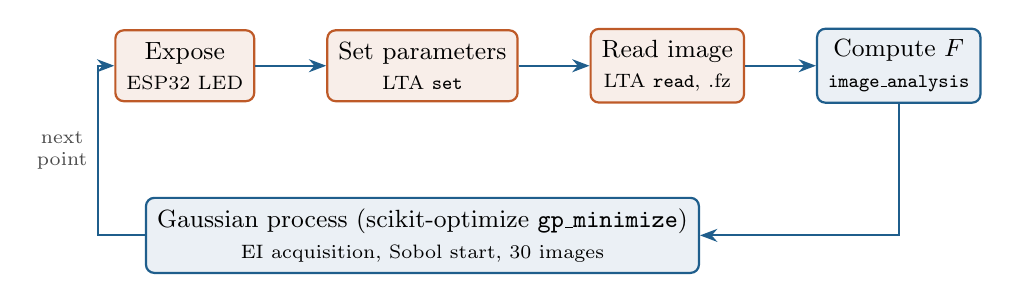
\begin{tikzpicture}[node distance=7mm and 9mm]
    \node[hw] (exp) {Expose\\\scriptsize ESP32 LED};
    \node[hw,right=of exp] (set) {Set parameters\\\scriptsize LTA \texttt{set}};
    \node[hw,right=of set] (read) {Read image\\\scriptsize LTA \texttt{read}, .fz};
    \node[box,right=of read] (f) {Compute $F$\\\scriptsize \texttt{image\_analysis}};
    \node[box,below=12mm of set,minimum width=60mm] (gp)
      {Gaussian process (scikit-optimize \texttt{gp\_minimize})\\
       \scriptsize EI acquisition, Sobol start, 30 images};
    \draw[arr] (exp) -- (set);
    \draw[arr] (set) -- (read);
    \draw[arr] (read) -- (f);
    \draw[arr] (f) |- (gp);
    \draw[arr] (gp.west) -- ++(-6mm,0) |- node[lbl,pos=0.25,left]{next\\point} (exp.west);
  \end{tikzpicture}

  \vspace{4mm}
  \begin{itemize}\small
    \item \texttt{optimize\_sensor\_LTA.py} plus three modules: \texttt{lta\_control} (hardware),
          \texttt{image\_analysis} (FITS + $F$), \texttt{bo\_core} (optimizer, CSV, plots)
    \item One JSON config per campaign; warm restart from a previous run
    \item These four files are kept unchanged throughout this work
  \end{itemize}
\end{frame}

% ===========================================================================
\section{Agentic version}
% ===========================================================================

\begin{frame}{Step 1: three cooperating agents}
  \centering
  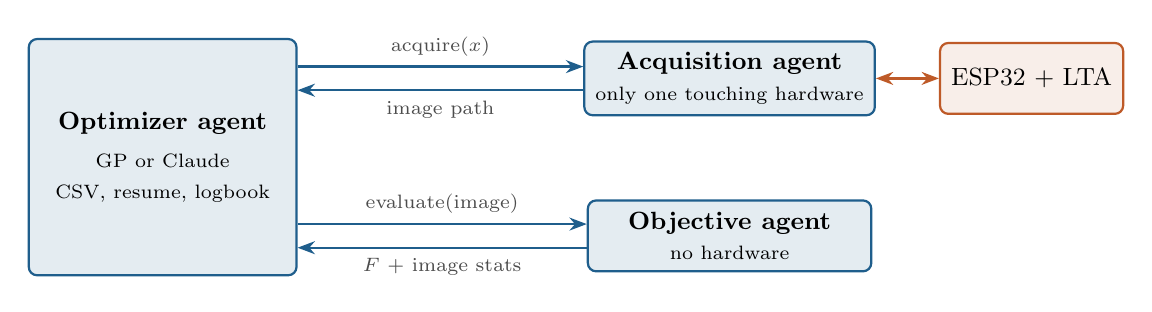
\begin{tikzpicture}
    \node[agent,minimum height=30mm,minimum width=34mm] (opt) at (0,0)
      {\textbf{Optimizer agent}\\[1mm]\scriptsize GP or Claude\\\scriptsize CSV, resume, logbook};
    \node[agent,minimum width=36mm] (acq) at (7.2,1.0)
      {\textbf{Acquisition agent}\\\scriptsize only one touching hardware};
    \node[agent,minimum width=36mm] (obj) at (7.2,-1.0)
      {\textbf{Objective agent}\\\scriptsize no hardware};
    \node[hw,right=8mm of acq] (hwn) {ESP32 + LTA};
    \coordinate (a1) at (0,1.15);  \coordinate (a2) at (0,0.85);
    \coordinate (b1) at (0,-0.85); \coordinate (b2) at (0,-1.15);
    \draw[arr] (opt.east |- a1) -- node[lbl,above]{acquire($x$)} (acq.west |- a1);
    \draw[arr] (acq.west |- a2) -- node[lbl,below]{image path} (opt.east |- a2);
    \draw[arr] (opt.east |- b1) -- node[lbl,above]{evaluate(image)} (obj.west |- b1);
    \draw[arr] (obj.west |- b2) -- node[lbl,below]{$F$ + image stats} (opt.east |- b2);
    \draw[{Stealth[length=2.2mm]}-{Stealth[length=2.2mm]},thick,draw=warm] (acq) -- (hwn);
  \end{tikzpicture}

  \vspace{3mm}
  \begin{itemize}\small
    \item Each agent is its own process (Python \texttt{multiprocessing}, standard library only)
    \item Messages are plain JSON dicts, all logged to \texttt{<run>\_messages.jsonl}
    \item New driver \texttt{optimize\_agents.py}: same config, options and output files
  \end{itemize}
\end{frame}

\begin{frame}[fragile]{Messages between agents}
\begin{lstlisting}
{"id": 7, "kind": "acquire", "sender": "optimizer",
 "payload": {"iteration": 3, "x_norm": [0.12, -0.40, 0.75, -0.05]}}

{"id": 8, "kind": "reply", "sender": "acquisition", "reply_to": 7, "ok": true,
 "payload": {"image_path": ".../optimize_76.fz"}}

{"id": 9, "kind": "evaluate", "sender": "optimizer",
 "payload": {"iteration": 3, "image_path": ".../optimize_76.fz"}}

{"id": 10, "kind": "reply", "sender": "objective", "reply_to": 9, "ok": true,
 "payload": {"F": 0.0296, "stats": {"noise_overscan": 636.4,
             "charge_overscan": 5310.0, "charge_active": 26812.5, "gain": 21502.5}}}
\end{lstlisting}
  \small
  \begin{itemize}
    \item The image statistics travel with every score: the GP ignores them, Claude uses them
    \item An agent error comes back as \texttt{"ok": false} with its traceback; the run stops cleanly
  \end{itemize}
\end{frame}

\begin{frame}{Validation: identical to the original}
  \begin{columns}[T]
    \begin{column}{0.55\textwidth}
      Simulated hardware for testing:
      \begin{itemize}\small
        \item fake \texttt{lta.sh}: synthetic images whose noise and signal depend on the voltages
        \item fake ESP32 and FITS reader, fake Claude
      \end{itemize}
      Original script vs.\ agent version, same config and seed:
      \begin{itemize}\small
        \item identical \texttt{gp\_results.csv}, progress CSV and images
        \item identical results on warm restart
      \end{itemize}
    \end{column}
    \begin{column}{0.42\textwidth}
      \begin{block}{Test suite}
        \small 29 automated tests, all passing\\[1mm]
        equivalence, messages, resume, failures, Claude optimizer, retries, cost,
        logbook
      \end{block}
      \vspace{2mm}
      {\scriptsize No hardware, network or API key needed:\\
       \texttt{python3 -m pytest tests}}
    \end{column}
  \end{columns}
\end{frame}

\begin{frame}{Running in the lab: the surrounding software matters}
  \small
  \begin{tabular}{p{0.28\textwidth}p{0.32\textwidth}p{0.32\textwidth}}
    \toprule
    Symptom & Cause & Fix \\
    \midrule
    ``No .fz image found'' & relative image path: Python and the LTA daemon resolved it from
      different directories & absolute \texttt{output\_base} in the config \\[1mm]
    Amplifiers mislabelled & config \texttt{amplifier} is the FITS HDU index; HDU 0 is empty &
      amplifier $N$ (0--3) $=$ \texttt{"amplifier": N+1}; recorded in every logbook entry \\[1mm]
    Claude run stopped after 16 images (\texttt{529 Overloaded}) & temporary API load &
      retries for up to $\sim$15 min \\[1mm]
    Interrupted runs could not be resumed & resume file written only at the end &
      \texttt{gp\_results.csv} written after every image \\
    \bottomrule
  \end{tabular}

  \vspace{3mm}
  Identifying the amplifier afterwards: recompute $F$ for every FITS extension of one image;
  only one reproduces the logged value.
\end{frame}

% ===========================================================================
\section{Claude as optimizer}
% ===========================================================================

\begin{frame}[fragile]{Step 2: Claude replaces the Gaussian process}
  \begin{columns}[T]
    \begin{column}{0.53\textwidth}
      \begin{enumerate}\small
        \item \textbf{Sobol start}: 8 space-filling points (as for the GP)
        \item \textbf{Each further point}: Claude (Opus 5.5) gets
          \begin{itemize}\scriptsize
            \item parameter descriptions, bounds, objective definition
            \item \emph{all} measurements so far, in physical units
            \item the image statistics ($\sigma_{os}$, $\sigma_{act}$, charges, gain),
                  which the GP never sees
            \item which amplifier is in use, operator notes, the logbook
          \end{itemize}
        \item Claude returns the next point as \textbf{structured JSON};
              values clipped to the bounds
      \end{enumerate}
    \end{column}
    \begin{column}{0.43\textwidth}
      \begin{block}{Drop-in replacement}
        \scriptsize \texttt{claude\_minimize()} has the interface of
        \texttt{gp\_minimize()} and returns the same result object: CSV, resume,
        pickle and plots unchanged. Switching is one line in the config.
      \end{block}
      \vspace{1mm}
\begin{lstlisting}
"optimizer": {
  "type": "claude",
  "n_calls": 30,
  "n_initial_points": 8,
  "model": "claude-opus-5-5",
  "effort": "high" }
\end{lstlisting}
    \end{column}
  \end{columns}
\end{frame}

\begin{frame}[fragile]{What Claude sees on each turn}
\begin{lstlisting}
Measurements so far (18):
# | Vdd | Vdrain | Vr | delay_H_overlap | F | noise_overscan | noise_active | charge_overscan | charge_active | gain
1 | -12.0 | -20.7 | -7.8 | 17.0 | 2.7763 | 869 | 920.6 | -1104 | -791 | 313
...
8 | -10.3 | -12.5 | -5.2 | 15.0 | 15.987 | 879.3 | 898.6 | -485 | -540 | -55
9 | -14.5 | -18.8 | -6.3 | 21.0 | 0.04715 | 682.7 | 1769 | 3365 | 1.784e+04 | 1.448e+04
...
18 | -17.5 | -20.2 | -5.0 | 30.0 | 0.02422 | 685.8 | 2456 | 6107 | 3.442e+04 | 2.832e+04

Measurements left in this campaign, including the next one: 12.
Choose the next point.
\end{lstlisting}
  \small
  Each iteration prints and logs (\texttt{<run>\_claude\_decisions.jsonl}):
  the proposed point, a \textbf{summary of Claude's thinking}, tokens and cost.

  \vspace{1mm}
  {\scriptsize Real rows (Oct 1, amplifier 2). Claude is never asked to write out its reasoning
   in the answer (Opus 5.5 declines that as ``reasoning extraction''); the explanation comes
   from the thinking summaries the API returns.}
\end{frame}

% ===========================================================================
\section{How Claude thinks and converges}
% ===========================================================================

\begin{frame}{How Claude thinks (1): using memory, noise and bounds}
  \small Real excerpts of the per-image thinking summaries, Oct 1:

  \vspace{1mm}
  \quoteblock{Re-checking a remembered best point (logbook)}{``The notebook's recorded best is
    (-14.5,-18.8,-6.3,21), so I should measure that point directly to verify reproducibility
    and use it as a reference.''\quad (It gave $F = 0.047$, not the remembered 0.019.)}
  \vspace{1mm}
  \quoteblock{Reasoning about noise and a parameter at its bound}{``The repeat of trial \#18
    showed noticeable noise ($\sim$0.01 variation) [\dots] I decide exploring Vr is valuable
    since we're sitting at a boundary value -- I'll test Vr around -5.6 to -6.0 [\dots] to
    confirm whether -5.0 is truly optimal or just unexplored territory.''}
  \vspace{1mm}
  \quoteblock{Noticing that the setup changed (broken amplifier 0)}{``These conditions look
    drastically different from before -- noise is much higher, F values are now in the 1.6-3
    range instead of 0.02-0.03 [\dots]''}
\end{frame}

\begin{frame}{How Claude thinks (2): learning the structure from scratch}
  \small Oct 2, GP vs.\ Claude comparison: Claude does \emph{not} read the logbook.

  \vspace{1mm}
  \quoteblock{Image 16: separating the parameters}{``I notice Vdd being more negative seems to
    help, while Vdrain is fairly flat between -10 and -13, so I want to test an edge case further
    out, maybe Vdrain -14.5 or -15 [\dots]''}
  \vspace{1mm}
  \quoteblock{Image 17: a parameter at its bound}{``The best region looks like Vdd=-23, Vr around
    -7.6/-7.7, delay 10, with Vdrain roughly flat between -10 and -15. I should explore further
    [\dots] since -23 seems to be at the boundary and already performing best.''}
  \vspace{1mm}
  \quoteblock{Its end-of-campaign logbook entry}{``Negative gain (\#2, \#3, \#5, \#7):
    charge\_active was below charge\_overscan, which is not a valid LED response. F uses |gain|,
    so these look deceptively moderate [\dots] Treat any gain $<$ 0 as a failure.''}
\end{frame}

\begin{frame}{How Claude converges: three amplifiers, Oct 1}
  \centering
  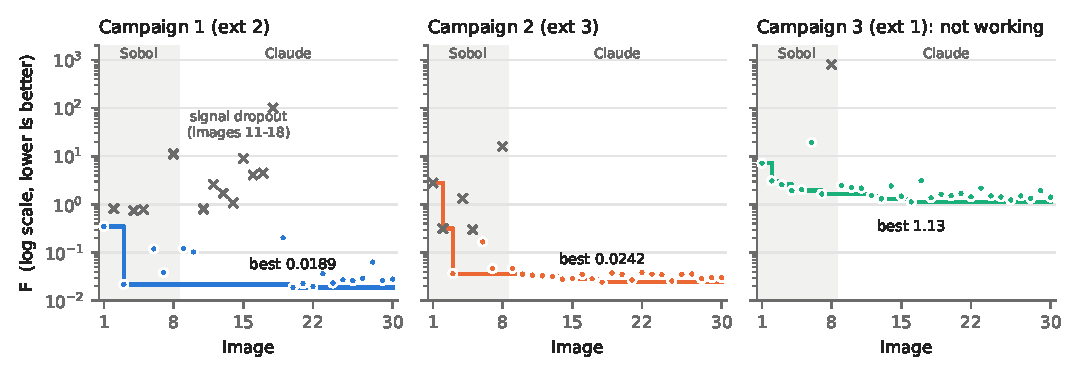
\includegraphics[width=0.97\textwidth]{figures/per_image_F.pdf}

  \vspace{1mm}
  \small
  \begin{itemize}
    \item Same 8 Sobol starting points, then 22 points chosen by Claude
    \item Converges within a few images after the start, then refines and re-measures
    \item Amplifier 0 was not working ($\sigma_{os}$ 50$\times$ higher); Claude flagged it
    \item Oct 1 illumination was mostly light leaks (operator note, Oct 2): signal $\sim 2\times10^4$ ADU
  \end{itemize}
\end{frame}

\begin{frame}{What Claude found: the $V_{dd}$--$V_{drain}$ relation (Oct 1)}
  \begin{columns}[T]
    \begin{column}{0.68\textwidth}
      \centering
      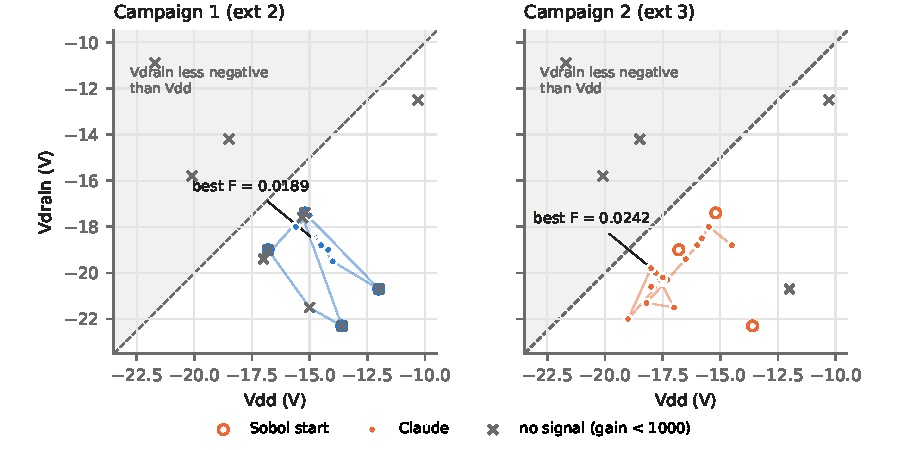
\includegraphics[width=\linewidth]{figures/vdd_vdrain.pdf}
    \end{column}
    \begin{column}{0.30\textwidth}
      \small
      \begin{itemize}
        \item Shaded: $V_{drain}$ less negative than $V_{dd}$ $\Rightarrow$ negative gain
        \item Good points: $V_{drain}$ 2.5--3\,V more negative than $V_{dd}$
        \item Claude's conclusion in the logbook:\\
              {\scriptsize\emph{``F is driven almost entirely by gain [\dots] most
              sensitive: the Vdd/Vdrain relationship''}}
      \end{itemize}
    \end{column}
  \end{columns}
\end{frame}

% ===========================================================================
\section{The lab logbook}
% ===========================================================================

\begin{frame}{The lab logbook: memory across campaigns}
  \centering
  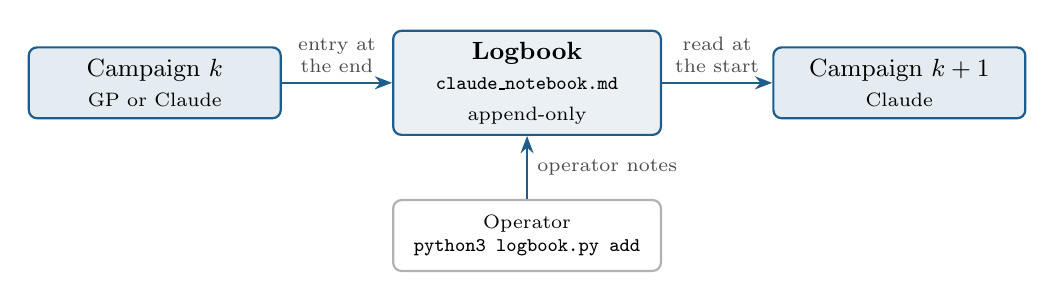
\begin{tikzpicture}[node distance=6mm and 14mm]
    \node[agent,minimum width=32mm] (run1) {Campaign $k$\\\scriptsize GP or Claude};
    \node[box,right=of run1,minimum width=34mm] (nb) {\textbf{Logbook}\\\scriptsize
      \texttt{claude\_notebook.md}\\\scriptsize append-only};
    \node[agent,right=of nb,minimum width=32mm] (run2) {Campaign $k+1$\\\scriptsize Claude};
    \node[note,below=8mm of nb,minimum width=34mm] (op) {Operator\\\texttt{python3 logbook.py add}};
    \draw[arr] (run1) -- node[lbl,above]{entry at\\the end} (nb);
    \draw[arr] (nb) -- node[lbl,above]{read at\\the start} (run2);
    \draw[arr] (op) -- node[lbl,right]{operator notes} (nb);
  \end{tikzpicture}

  \vspace{3mm}
  \begin{itemize}\small
    \item Each API call starts from scratch: Claude does not learn between runs by itself
    \item \textbf{Every run} (GP, Claude, interrupted) appends an entry
    \item Claude reads it at the start as \emph{prior knowledge}; current measurements take
          priority, and a later entry overrides an earlier one
    \item \textbf{Append-only}: entries are never changed; corrections are new entries
  \end{itemize}
\end{frame}

\begin{frame}[fragile]{Anatomy of an entry (Oct 2, Claude run)}
\begin{lstlisting}
## 2026-10-02 17:46 | module skipper | amp 3 (HDU 4) | claude | 30 measurements (30 new) |
   best F = 0.42845 at Vdd=-23.0, Vdrain=-10.5, Vr=-7.4, delay_H_overlap=10.0

**Run facts** (recorded by the code)
- Optimizer: claude; config: config_compare_claude.json; images optimize_424.fz to
  optimize_453.fz; 17:36-17:46.
- Best F this run: 0.4284 at (Vdd=-23.0, Vdrain=-10.5, Vr=-7.4, delay_H_overlap=10.0), [...]
- Signal (gain, ADU): median 1177, max 1590; [...]
- Overscan noise (ADU): median 693, range 614-943.

**Best region.** The best results came from Vdd = -23.0, Vdrain = -10.5, Vr = -7.4 and
delay_H_overlap = 10. [...] Repeat scatter is about +-0.03-0.05.
**Sensitivity.** F is driven mainly by gain. Vdd had the largest effect [...]
**Suggestions for the next campaign.** [...] Both Vdd and delay are pinned at their bounds.
If hardware limits permit, extend Vdd below -23 and delay below 10 and test there first.
\end{lstlisting}
  \small
  \begin{itemize}
    \item \textbf{Header + run facts}: written by the code for every run (facts, not opinions)
    \item \textbf{Analysis}: written by Claude for Claude runs
  \end{itemize}
\end{frame}

\begin{frame}[fragile]{Using the logbook}
  \begin{columns}[T]
    \begin{column}{0.55\textwidth}
\begin{lstlisting}
python3 logbook.py list           # one line per entry
python3 logbook.py show           # latest entry
python3 logbook.py show 3 5       # entries 3 and 5
python3 logbook.py search dropout
python3 logbook.py add --amp 3 -m "LED replaced"
python3 logbook.py add --amp 3    # write it in the editor
\end{lstlisting}
      \small
      \begin{itemize}
        \item Config: \texttt{"notebook\_read": false} --- Claude does not read it
              (fair comparisons) but the entry is still written
        \item \texttt{"notebook": false} --- off completely
      \end{itemize}
    \end{column}
    \begin{column}{0.42\textwidth}
      \begin{block}{A real operator note (Oct 2)}
        \scriptsize\emph{``I think the optimization that we did yesterday 10/1/2026 were using
        as illumination a lot of light leaks on the system. Now I am using as illumination the
        LED, I closed most of the light leaks. I think that is why the ``gain'' [\dots] is much
        lower than before.''}
      \end{block}
      {\scriptsize Marked \texttt{operator note}; Claude treats these as first-hand observations.}
    \end{column}
  \end{columns}
\end{frame}

\begin{frame}{What the logbook caught}
  \begin{itemize}
    \item \textbf{A broken amplifier} (Oct 1): \emph{``Setup state changed sharply this
          campaign [\dots] noise\_overscan was 3.1--4.5e4 ADU, about 50$\times$ [\dots] F values
          from this campaign are not comparable with earlier entries.''}
    \item \textbf{Signal decay} (Oct 2, 15:15): gain halving image after image;
          \emph{``When the reference gain starts to decay, stop optimizing and investigate the
          LED or exposure chain''}
    \item \textbf{Its own limits}: the shared logbook did not record the amplifier, so Claude
          could only guess (``hardware, offset or cabling''). Fixed: every entry now records it,
          and Claude is told which amplifier is in use
    \item \textbf{Illumination change}: the operator note on light leaks explains why the Oct 2
          signal is $\sim$15$\times$ lower --- and changed how we read later runs
  \end{itemize}
\end{frame}

% ===========================================================================
\section{GP vs.\ Claude}
% ===========================================================================

\begin{frame}{Comparison setup}
  \begin{columns}[T]
    \begin{column}{0.55\textwidth}
      \begin{itemize}
        \item Same session, back to back (Oct 2): GP 17:28--17:36, Claude 17:36--17:46
        \item Same amplifier: amp 3 (\texttt{-{}-amplifier 4}), LED-only illumination
        \item Same budget: 30 images, 8 Sobol + 22 guided
        \item Same agents and objective; only the optimizer differs
        \item Claude does \textbf{not} read the logbook: no prior knowledge
      \end{itemize}
    \end{column}
    \begin{column}{0.42\textwidth}
      \begin{block}{Commands}
        \scriptsize\ttfamily python3 optimize\_agents.py \textbackslash\\
        \ \ -{}-config config\_compare\_gp.json \textbackslash\\
        \ \ -{}-amplifier 4\\[1mm]
        python3 optimize\_agents.py \textbackslash\\
        \ \ -{}-config config\_compare\_claude.json \textbackslash\\
        \ \ -{}-amplifier 4
      \end{block}
    \end{column}
  \end{columns}
\end{frame}

\begin{frame}{Results}
  \small
  \begin{tabular}{p{0.22\textwidth}p{0.33\textwidth}p{0.37\textwidth}}
    \toprule
    & \textcolor{gpblue}{\textbf{GP}} & \textcolor{clorange}{\textbf{Claude}} \\
    \midrule
    Best $F$ (any sign) & 0.769 at $(-23,\,-23,\,-6.7,\,30)$ & \textbf{0.428} at $(-23,\,-10.5,\,-7.4,\,10)$ \\
    Gain at that point & \textbf{$-$1054 ADU} (inverted) & $+$1590 ADU \\
    Best $F$ with gain $>0$ & 0.920 (gain 850) & \textbf{0.428} (gain 1590) \\
    Images with gain $>0$ & 14 of 30 (10 of 22 guided) & 26 of 30 (all 22 guided; 20 above 900 ADU) \\
    Behaviour & guided points mostly at the bounds & region found by image 10, then refined \\
    Repeatability at best point & --- & 6 images: $F = 0.43$--$0.52$ \\
    Time / cost & 8 min / free & 10 min / \$0.28 \\
    \bottomrule
  \end{tabular}

  \vspace{3mm}
  \begin{itemize}
    \item Among valid (positive-gain) images Claude reaches $\sim$2$\times$ lower $F$ with
          $\sim$2$\times$ more signal
    \item The GP's ``best'' image is an inverted signal: it optimized $|\text{gain}|$
  \end{itemize}
\end{frame}

\begin{frame}{Every image: score and signal}
  \centering
  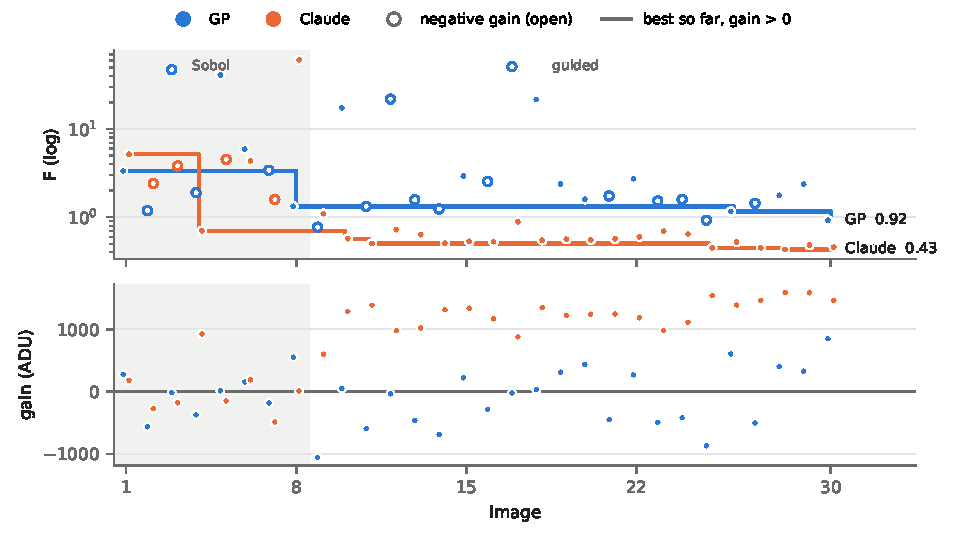
\includegraphics[width=0.86\textwidth]{figures/compare_per_image.pdf}

  \small
  Top: $F$ per image; line = best so far among positive-gain images.
  Bottom: signal (gain). Claude finds a region of consistent positive signal; the GP keeps
  jumping between positive and negative gain.
\end{frame}

\begin{frame}{How each method moves through the parameter space}
  \centering
  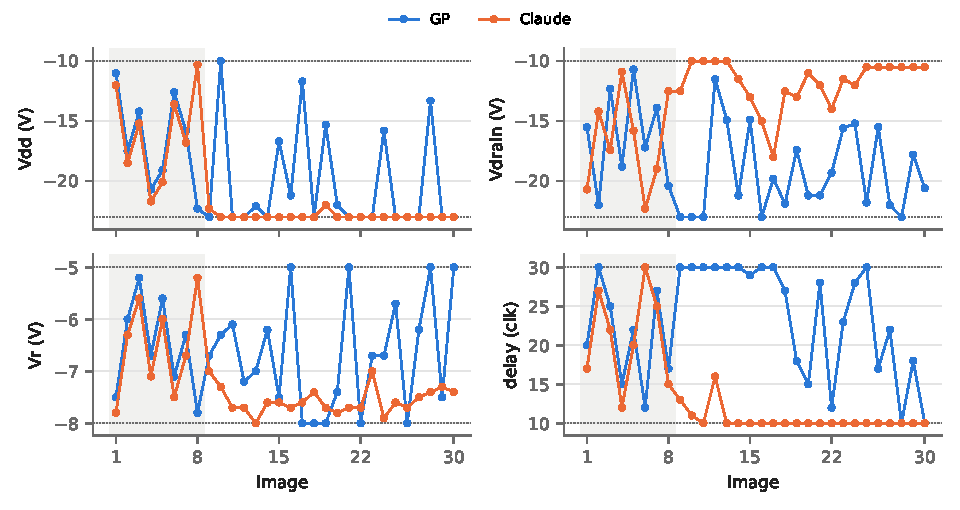
\includegraphics[width=0.8\textwidth]{figures/compare_trajectories.pdf}

  \small
  Dotted lines: bounds. Claude converges to $V_{dd}=-23$, $V_{drain}\approx-10.5$,
  $V_r\approx-7.5$, delay $=10$ and then explores \emph{one parameter at a time} around it;
  the GP keeps sampling the edges of the space.
\end{frame}

\begin{frame}{Is the LED signal real? The shot-noise check}
  \begin{columns}[T]
    \begin{column}{0.48\textwidth}
      \centering
      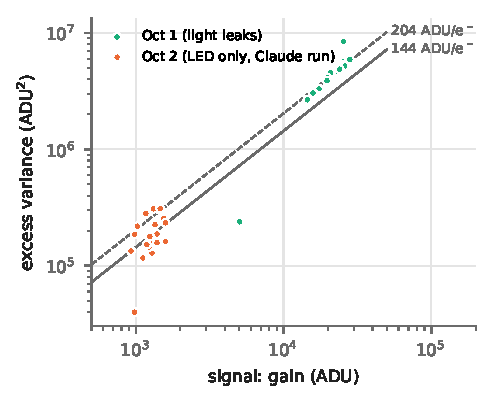
\includegraphics[width=\linewidth]{figures/shot_noise.pdf}
    \end{column}
    \begin{column}{0.50\textwidth}
      \small
      \begin{itemize}
        \item Light adds photon shot noise: excess variance
              $\sigma_{act}^2 - \sigma_{os}^2 \approx k \cdot S$
        \item Oct 1 (light leaks): $k \approx 204$ ADU/e$^-$, $S \sim 2\times10^4$ ADU
        \item Oct 2 (LED only, Claude's region): $k \approx 144$ ADU/e$^-$, $S \sim 1.4\times10^3$ ADU
        \item Same order of $k$ $\Rightarrow$ the small Oct 2 signal is real light,
              $\sim$10 e$^-$ per pixel --- not an offset
      \end{itemize}
    \end{column}
  \end{columns}
\end{frame}

\begin{frame}{Why the GP lost, and a second pair that agrees}
  \begin{itemize}
    \item $F$ uses $|\text{gain}|$: an inverted signal looks as good as a real one
          \begin{itemize}\small
            \item the GP minimizes $F$ blindly and ranked an inverted image first
            \item Claude sees the statistics and concluded, unprompted:
                  \emph{``Treat any gain $<$ 0 as a failure''}
          \end{itemize}
    \item With weak signal, $F$ is noisy and nearly flat over most of the space: hard for a GP
          with no notion of what a valid image is
  \end{itemize}

  \vspace{2mm}
  \small
  \begin{tabular}{p{0.28\textwidth}p{0.30\textwidth}p{0.34\textwidth}}
    \toprule
    Earlier pair, Oct 2 & GP (16:09) & Claude (16:19) \\
    \midrule
    Best $F$ & 0.878 & \textbf{0.440} \\
    at $(V_{dd}, V_{drain}, V_r,$ delay) & $(-16.5,\,-10.0,\,-5.0,\,10)$ & $(-19.5,\,-10.5,\,-7.4,\,11)$ \\
    \bottomrule
  \end{tabular}

  \vspace{1mm}
  Claude reached the same corner ($V_{drain}\approx-10.5$, $V_r\approx-7.5$, delay $\approx 10$)
  in both runs, with $F = 0.44$ and $0.43$.
\end{frame}

\begin{frame}{Cost}
  \begin{columns}[T]
    \begin{column}{0.5\textwidth}
      \small
      \begin{tabular}{lr}
        \toprule
        Claude Opus 5.5 (list price) & per M tokens \\
        \midrule
        input & \$4.00 \\
        output (incl.\ thinking) & \$20.00 \\
        cached input, read & \$0.20 \\
        \bottomrule
      \end{tabular}

      \vspace{3mm}
      \begin{tabular}{lr}
        \toprule
        Campaign (22 decisions) & cost \\
        \midrule
        Oct 1, amplifiers 1, 2, 0 & \$0.31, \$0.31, \$0.39 \\
        Oct 2, 16:19 & \$0.27 \\
        Oct 2, 17:36 (comparison) & \$0.28 \\
        \bottomrule
      \end{tabular}
      {\scriptsize\\ List-price estimates; plus one logbook-entry request per campaign.}
    \end{column}
    \begin{column}{0.46\textwidth}
      \begin{itemize}\small
        \item Tracked automatically: tokens and cost per image, running total, summary
        \item $\approx$\$0.01--0.02 per decision, $\approx$\$0.3 per 10-minute campaign
        \item Small compared to the lab time per image
      \end{itemize}
    \end{column}
  \end{columns}
\end{frame}

% ===========================================================================
\section{Lessons}
% ===========================================================================

\begin{frame}{Gaussian process vs.\ Claude}
  \small
  \begin{tabular}{p{0.24\textwidth}p{0.33\textwidth}p{0.33\textwidth}}
    \toprule
    & Gaussian process & Claude \\
    \midrule
    Information used & parameters and $F$ only & $F$, image statistics, notes, logbook \\
    Validity of an image & unknown to it & reasons about it (e.g.\ negative gain) \\
    Reproducible & yes (fixed seed) & no, but it re-measures to estimate noise \\
    Explains choices & no & thinking summary per image, logbook entry \\
    Memory across runs & warm restart (data only) & data + written lessons \\
    Cost & free & $\sim$\$0.3 per campaign \\
    Failure modes & outliers, flat/noisy $F$, inverted signals & API availability, safety filters \\
    \bottomrule
  \end{tabular}

  \vspace{3mm}
  Same agents, same outputs: switching is one line in the config.
\end{frame}

\begin{frame}{Lessons and next steps}
  \begin{itemize}
    \item \textbf{Fix the objective for both}: reject or penalize gain $\le 0$ (the
          \texttt{negative\_gain} penalty exists, currently off); the GP should not win with
          an inverted image
    \item \textbf{Extend the bounds}: $V_{dd}$ and delay ended at their limits ($-23$\,V, 10\,clk)
    \item \textbf{Repeat the comparison} with the corrected objective and new bounds, and on a
          second amplifier
    \item \textbf{Noise of $F$}: repeated images at a fixed point, to state which differences
          are real
    \item \textbf{Stopping rule}: today a fixed budget of 30 images
    \item \textbf{Better objective}: e.g.\ ``best flat field for astronomy'', with criteria drawn
          from the literature and reviewed before use
  \end{itemize}
\end{frame}

\begin{frame}{Summary}
  \begin{enumerate}
    \item Started from a GP optimizer for the Skipper-CCD operating point
    \item Rebuilt it as three agents (acquisition, objective, optimizer), verified identical
    \item Replaced the GP by Claude as a drop-in: it uses the image statistics and explains
          every choice
    \item Added a lab logbook: every run appends facts (and Claude's analysis); Claude reads it
          as memory; operators add notes; append-only
    \item Same-session comparison on one amplifier: Claude found a consistent positive-signal
          region with $\sim$2$\times$ lower $F$; the GP's best image was an inverted signal
  \end{enumerate}
  \vspace{3mm}
  \centering
  {\small Code: \texttt{optimize\_agents.py}, \texttt{agents/}, \texttt{logbook.py}, \texttt{tests/}}
\end{frame}

\end{document}
